% Created by tikzDevice version 0.12.3.1 on 2021-07-06 13:53:03
% !TEX encoding = UTF-8 Unicode
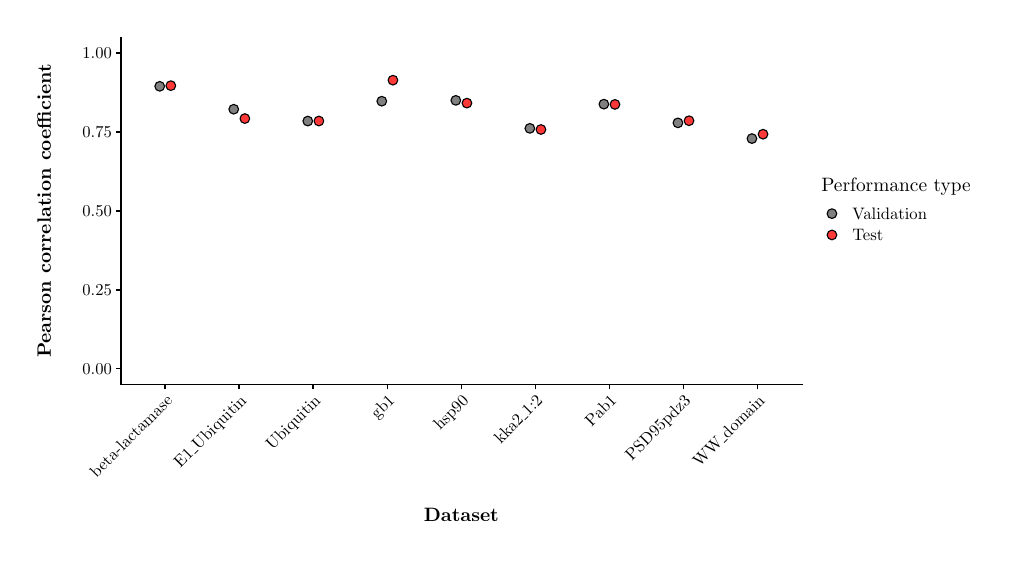
\begin{tikzpicture}[x=1pt,y=1pt]
\definecolor{fillColor}{RGB}{255,255,255}
\path[use as bounding box,fill=fillColor,fill opacity=0.00] (0,0) rectangle (344.26,183.39);
\begin{scope}
\path[clip] ( 33.67, 54.47) rectangle (279.77,179.89);
\definecolor{drawColor}{RGB}{0,0,0}
\definecolor{fillColor}{RGB}{128,128,128}

\path[draw=drawColor,line width= 0.4pt,line join=round,line cap=round,fill=fillColor] ( 74.46,153.92) circle (  1.75);
\definecolor{fillColor}{RGB}{255,56,56}

\path[draw=drawColor,line width= 0.4pt,line join=round,line cap=round,fill=fillColor] ( 78.48,150.55) circle (  1.75);
\definecolor{fillColor}{RGB}{128,128,128}

\path[draw=drawColor,line width= 0.4pt,line join=round,line cap=round,fill=fillColor] (234.96,148.99) circle (  1.75);
\definecolor{fillColor}{RGB}{255,56,56}

\path[draw=drawColor,line width= 0.4pt,line join=round,line cap=round,fill=fillColor] (238.97,149.76) circle (  1.75);
\definecolor{fillColor}{RGB}{128,128,128}

\path[draw=drawColor,line width= 0.4pt,line join=round,line cap=round,fill=fillColor] (208.21,155.75) circle (  1.75);
\definecolor{fillColor}{RGB}{255,56,56}

\path[draw=drawColor,line width= 0.4pt,line join=round,line cap=round,fill=fillColor] (212.22,155.66) circle (  1.75);
\definecolor{fillColor}{RGB}{128,128,128}

\path[draw=drawColor,line width= 0.4pt,line join=round,line cap=round,fill=fillColor] (101.21,149.64) circle (  1.75);
\definecolor{fillColor}{RGB}{255,56,56}

\path[draw=drawColor,line width= 0.4pt,line join=round,line cap=round,fill=fillColor] (105.23,149.66) circle (  1.75);
\definecolor{fillColor}{RGB}{128,128,128}

\path[draw=drawColor,line width= 0.4pt,line join=round,line cap=round,fill=fillColor] (261.71,143.31) circle (  1.75);
\definecolor{fillColor}{RGB}{255,56,56}

\path[draw=drawColor,line width= 0.4pt,line join=round,line cap=round,fill=fillColor] (265.72,144.89) circle (  1.75);
\definecolor{fillColor}{RGB}{128,128,128}

\path[draw=drawColor,line width= 0.4pt,line join=round,line cap=round,fill=fillColor] ( 47.71,162.20) circle (  1.75);
\definecolor{fillColor}{RGB}{255,56,56}

\path[draw=drawColor,line width= 0.4pt,line join=round,line cap=round,fill=fillColor] ( 51.73,162.44) circle (  1.75);
\definecolor{fillColor}{RGB}{128,128,128}

\path[draw=drawColor,line width= 0.4pt,line join=round,line cap=round,fill=fillColor] (127.96,156.82) circle (  1.75);
\definecolor{fillColor}{RGB}{255,56,56}

\path[draw=drawColor,line width= 0.4pt,line join=round,line cap=round,fill=fillColor] (131.98,164.41) circle (  1.75);
\definecolor{fillColor}{RGB}{128,128,128}

\path[draw=drawColor,line width= 0.4pt,line join=round,line cap=round,fill=fillColor] (154.71,157.12) circle (  1.75);
\definecolor{fillColor}{RGB}{255,56,56}

\path[draw=drawColor,line width= 0.4pt,line join=round,line cap=round,fill=fillColor] (158.72,156.13) circle (  1.75);
\definecolor{fillColor}{RGB}{128,128,128}

\path[draw=drawColor,line width= 0.4pt,line join=round,line cap=round,fill=fillColor] (181.46,147.01) circle (  1.75);
\definecolor{fillColor}{RGB}{255,56,56}

\path[draw=drawColor,line width= 0.4pt,line join=round,line cap=round,fill=fillColor] (185.47,146.59) circle (  1.75);
\end{scope}
\begin{scope}
\path[clip] (  0.00,  0.00) rectangle (344.26,183.39);
\definecolor{drawColor}{RGB}{0,0,0}

\path[draw=drawColor,line width= 0.6pt,line join=round,line cap=rect] ( 33.67, 54.47) --
	( 33.67,179.89);
\end{scope}
\begin{scope}
\path[clip] (  0.00,  0.00) rectangle (344.26,183.39);
\definecolor{drawColor}{RGB}{0,0,0}

\node[text=drawColor,anchor=base east,inner sep=0pt, outer sep=0pt, scale=  0.60] at ( 30.42, 58.11) {0.00};

\node[text=drawColor,anchor=base east,inner sep=0pt, outer sep=0pt, scale=  0.60] at ( 30.42, 86.61) {0.25};

\node[text=drawColor,anchor=base east,inner sep=0pt, outer sep=0pt, scale=  0.60] at ( 30.42,115.11) {0.50};

\node[text=drawColor,anchor=base east,inner sep=0pt, outer sep=0pt, scale=  0.60] at ( 30.42,143.62) {0.75};

\node[text=drawColor,anchor=base east,inner sep=0pt, outer sep=0pt, scale=  0.60] at ( 30.42,172.12) {1.00};
\end{scope}
\begin{scope}
\path[clip] (  0.00,  0.00) rectangle (344.26,183.39);
\definecolor{drawColor}{RGB}{0,0,0}

\path[draw=drawColor,line width= 0.6pt,line join=round] ( 31.92, 60.17) --
	( 33.67, 60.17);

\path[draw=drawColor,line width= 0.6pt,line join=round] ( 31.92, 88.68) --
	( 33.67, 88.68);

\path[draw=drawColor,line width= 0.6pt,line join=round] ( 31.92,117.18) --
	( 33.67,117.18);

\path[draw=drawColor,line width= 0.6pt,line join=round] ( 31.92,145.68) --
	( 33.67,145.68);

\path[draw=drawColor,line width= 0.6pt,line join=round] ( 31.92,174.19) --
	( 33.67,174.19);
\end{scope}
\begin{scope}
\path[clip] (  0.00,  0.00) rectangle (344.26,183.39);
\definecolor{drawColor}{RGB}{0,0,0}

\path[draw=drawColor,line width= 0.6pt,line join=round,line cap=rect] ( 33.67, 54.47) --
	(279.77, 54.47);
\end{scope}
\begin{scope}
\path[clip] (  0.00,  0.00) rectangle (344.26,183.39);
\definecolor{drawColor}{RGB}{0,0,0}

\path[draw=drawColor,line width= 0.6pt,line join=round] ( 49.72, 52.72) --
	( 49.72, 54.47);

\path[draw=drawColor,line width= 0.6pt,line join=round] ( 76.47, 52.72) --
	( 76.47, 54.47);

\path[draw=drawColor,line width= 0.6pt,line join=round] (103.22, 52.72) --
	(103.22, 54.47);

\path[draw=drawColor,line width= 0.6pt,line join=round] (129.97, 52.72) --
	(129.97, 54.47);

\path[draw=drawColor,line width= 0.6pt,line join=round] (156.72, 52.72) --
	(156.72, 54.47);

\path[draw=drawColor,line width= 0.6pt,line join=round] (183.47, 52.72) --
	(183.47, 54.47);

\path[draw=drawColor,line width= 0.6pt,line join=round] (210.22, 52.72) --
	(210.22, 54.47);

\path[draw=drawColor,line width= 0.6pt,line join=round] (236.97, 52.72) --
	(236.97, 54.47);

\path[draw=drawColor,line width= 0.6pt,line join=round] (263.72, 52.72) --
	(263.72, 54.47);
\end{scope}
\begin{scope}
\path[clip] (  0.00,  0.00) rectangle (344.26,183.39);
\definecolor{drawColor}{RGB}{0,0,0}

\node[text=drawColor,rotate= 45.00,anchor=base east,inner sep=0pt, outer sep=0pt, scale=  0.60] at ( 52.64, 48.30) {beta-lactamase};

\node[text=drawColor,rotate= 45.00,anchor=base east,inner sep=0pt, outer sep=0pt, scale=  0.60] at ( 79.39, 48.30) {E1\_Ubiquitin};

\node[text=drawColor,rotate= 45.00,anchor=base east,inner sep=0pt, outer sep=0pt, scale=  0.60] at (106.14, 48.30) {Ubiquitin};

\node[text=drawColor,rotate= 45.00,anchor=base east,inner sep=0pt, outer sep=0pt, scale=  0.60] at (132.89, 48.30) {gb1};

\node[text=drawColor,rotate= 45.00,anchor=base east,inner sep=0pt, outer sep=0pt, scale=  0.60] at (159.64, 48.30) {hsp90};

\node[text=drawColor,rotate= 45.00,anchor=base east,inner sep=0pt, outer sep=0pt, scale=  0.60] at (186.39, 48.30) {kka2\_1:2};

\node[text=drawColor,rotate= 45.00,anchor=base east,inner sep=0pt, outer sep=0pt, scale=  0.60] at (213.14, 48.30) {Pab1};

\node[text=drawColor,rotate= 45.00,anchor=base east,inner sep=0pt, outer sep=0pt, scale=  0.60] at (239.89, 48.30) {PSD95pdz3};

\node[text=drawColor,rotate= 45.00,anchor=base east,inner sep=0pt, outer sep=0pt, scale=  0.60] at (266.64, 48.30) {WW\_domain};
\end{scope}
\begin{scope}
\path[clip] (  0.00,  0.00) rectangle (344.26,183.39);
\definecolor{drawColor}{RGB}{0,0,0}

\node[text=drawColor,anchor=base,inner sep=0pt, outer sep=0pt, scale=  0.70] at (156.72,  4.86) {\bfseries Dataset};
\end{scope}
\begin{scope}
\path[clip] (  0.00,  0.00) rectangle (344.26,183.39);
\definecolor{drawColor}{RGB}{0,0,0}

\node[text=drawColor,rotate= 90.00,anchor=base,inner sep=0pt, outer sep=0pt, scale=  0.70] at (  8.39,117.18) {\bfseries Pearson correlation coefficient};
\end{scope}
\begin{scope}
\path[clip] (  0.00,  0.00) rectangle (344.26,183.39);
\definecolor{drawColor}{RGB}{0,0,0}

\node[text=drawColor,anchor=base west,inner sep=0pt, outer sep=0pt, scale=  0.70] at (286.77,124.22) {Performance type};
\end{scope}
\begin{scope}
\path[clip] (  0.00,  0.00) rectangle (344.26,183.39);
\definecolor{drawColor}{RGB}{0,0,0}
\definecolor{fillColor}{RGB}{128,128,128}

\path[draw=drawColor,line width= 0.4pt,line join=round,line cap=round,fill=fillColor] (290.62,116.19) circle (  1.75);
\end{scope}
\begin{scope}
\path[clip] (  0.00,  0.00) rectangle (344.26,183.39);
\definecolor{drawColor}{RGB}{0,0,0}
\definecolor{fillColor}{RGB}{255,56,56}

\path[draw=drawColor,line width= 0.4pt,line join=round,line cap=round,fill=fillColor] (290.62,108.49) circle (  1.75);
\end{scope}
\begin{scope}
\path[clip] (  0.00,  0.00) rectangle (344.26,183.39);
\definecolor{drawColor}{RGB}{0,0,0}

\node[text=drawColor,anchor=base west,inner sep=0pt, outer sep=0pt, scale=  0.60] at (297.97,114.12) {Validation};
\end{scope}
\begin{scope}
\path[clip] (  0.00,  0.00) rectangle (344.26,183.39);
\definecolor{drawColor}{RGB}{0,0,0}

\node[text=drawColor,anchor=base west,inner sep=0pt, outer sep=0pt, scale=  0.60] at (297.97,106.42) {Test};
\end{scope}
\end{tikzpicture}
